%!TEX root = paper.tex
\section{Countermeasures}
\label{sec:countermeasures}

\begin{figure}[t!]
    \centering
    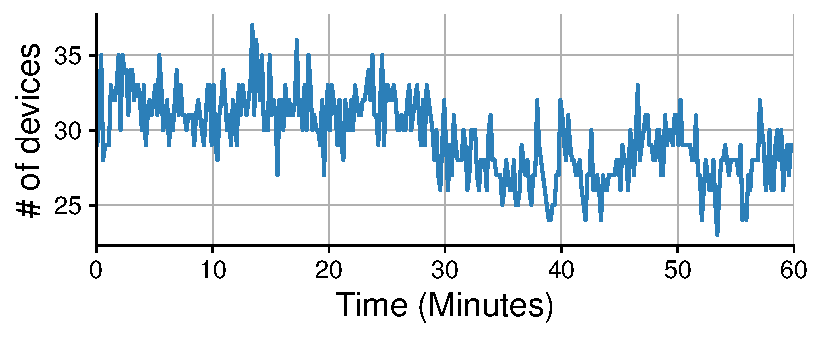
\includegraphics[width = \linewidth]{bletracking/plots/case_study_android_devno2.pdf} 
    \caption{Number of unique MAC addresses observed over time while tracking the target.}
    \label{fig:android_no}
\end{figure}

BLE location tracking based on hardware impairments cannot be defended against by simple software/firmware update
mechanisms. These manufacturing variation based properties
are baked into the RF signal chain.
%; as long as the device transmits the signal will have CFO and I/Q offset and imbalance.

One possible defense against this attack requires us to rethink the design of a BLE chipset's signal chain.
%
We envision adding a random time-varying extra frequency offset the crystal oscillator.
%
This would cause the CFO measured at the receiver to also be time-varying and unpredictable.
%
Fortunately, since BLE has a large CFO tolerance (150 kHz~\cite{btcorespec}), an extra frequency shift will not impact packet decoding.
%
%However, our attacker who relies on a stable CFO to track the target, will no longer be able to utilize these hardware impairments as a reliable identifier.

We also envision another defense that does not require hardware modification.
%
In Section~\ref{sec:challenges:temperature} we observed that CFO changes significantly when a device's internal components heat up and cool down.
%
Internal component temperature depends on the workload running on the phone: a time-varying workload can result in a time-varying CFO.
%
We envision a defense in which a background process runs a computation, and keeps randomly changing the computation in line with the MAC address changes.
%
Unfortunately, a constantly changing workload can result in a constantly changing battery consumption.
%
Worse still, if the device temperature remains constantly elevated, the battery life also decreases over time~\cite{fireinyourhands}.

\begin{comment}
We envision the following possible countermeasures to defend against the location tracking attack.
%
Since CFO is the major contributor to BLE device identification (Section~\ref{sec:results:field}), we focus our defenses on manipulating this property only.
%



\subsection{Modifying the crystal oscillator circuit}
\noteby{NB}{
As we have seen, for any BLE chipset the CFO imperfection arises in the crystal oscillator circuit of the BLE radio.
%
The mobile device is identifiable because the CFO imperfection is unique to any BLE radio.
%
Therefore, we can envision the design of a new crystal oscillator circuit that adds a fake CFO beyond the inherent CFO imperfection
}

\subsubsection*{Limitations}
\noteby{NB}{
Implementing something like this would require a complete redesign of the BLE radio chipsets, which is time-consuming and costly.
%
Additionally, this solution only benefits future BLE radios. 
%
The millions of phones already in operation will still use the unmodified BLE radios and will remain vulnerable to the tracking attack.
}
\end{comment}
